% 1  Introduction
\section{Introduction}

% 1.1  Define tsunami wave (versus wind wave)
	\slide[Tsunami Waves] {
	\begin{enumerate}
		\item Tsunami waves are long waves, $\lambda>> D$ or $\frac{D}{\lambda}\approx0$.
		
		\item Wind waves are short waves, $\lambda\not>\not> D$ or $\frac{D}{\lambda}\not\approx 0$.
		\end{enumerate}
		\centering
		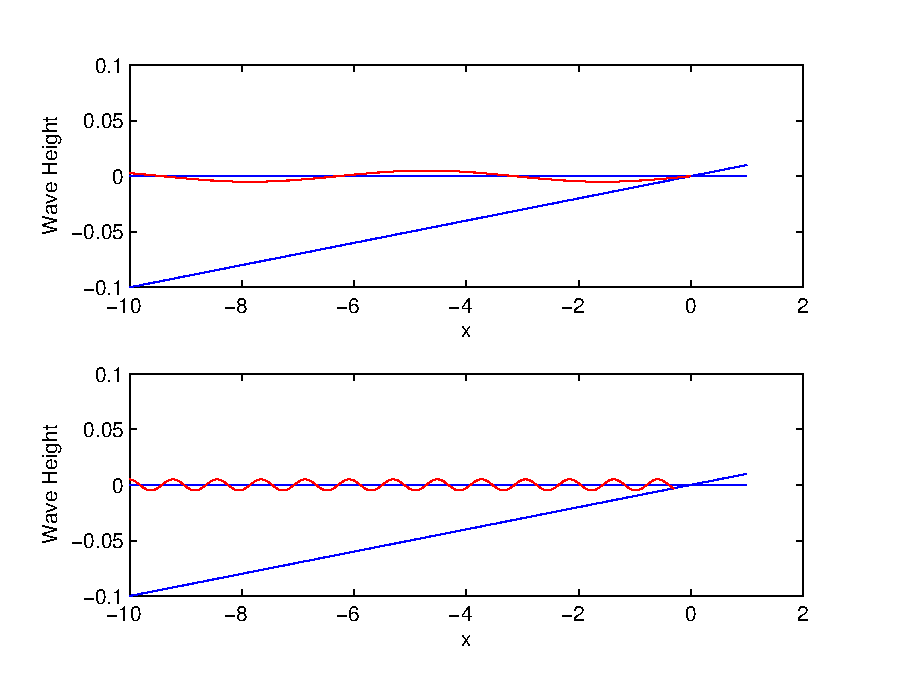
\includegraphics[width=.8\textwidth]{bay/wave_comp.eps}
	}
% 1.1.1  Typical causes of tsunami waves
	\slide[Causes of Tsunami Waves] {
	\begin{tabular}{|l|l|}\hline
		Rock Slides--Chehalis Lake&Earthquakes\\
			 \includegraphics[width=.4\textwidth]{causes/Landslide.jpg}%http://wikimapia.org/22797805/Chehalis-Lake-Rock-Slide
			&\includegraphics[width=.5\textwidth]{causes/Earrthquake.png}\\\hline%http://www.enchantedlearning.com/subjects/tsunami/\\\hline
			Asteroid Impact&Glacier Calving\\
			 ~ ~ \includegraphics[width=.3\textwidth]{causes/Asteroid.jpg}%http://mail.colonial.net/~hkaiter/asteroidbelt.html
			&\includegraphics[width=.5\textwidth]{causes/Calving.jpg}\\\hline
	\end{tabular}
	}


\slide[Purpose of Research]{
\bi
	\item Model run-up for the closed bays with a steep wall.
	\item Understand basic run-up properties of different bays.
\ei
}
% 1.1.2  Include pictures/videos ? from trip and elsewhere
% 1.2  Purpose of our research
	\slide[Introduction to the Problem]{
		Mathematical modeling of tsunami run-up.
		\bi	\item Numerous real-world applications.
			\item Analytical solutions allow numerical solutions to be checked.
			\item Primarily involves solving non-linear partial differential equations.
		\ei
		Our REU program focused on
		\bi	\item Bays of U-Shaped bays of finite length.
			\item Used a spectral method to find numerical series solutions.
		\ei
	}